\chapter{Proteus}

    \section{Schéma}

        \begin{figure}[!h]
            \begin{center}
                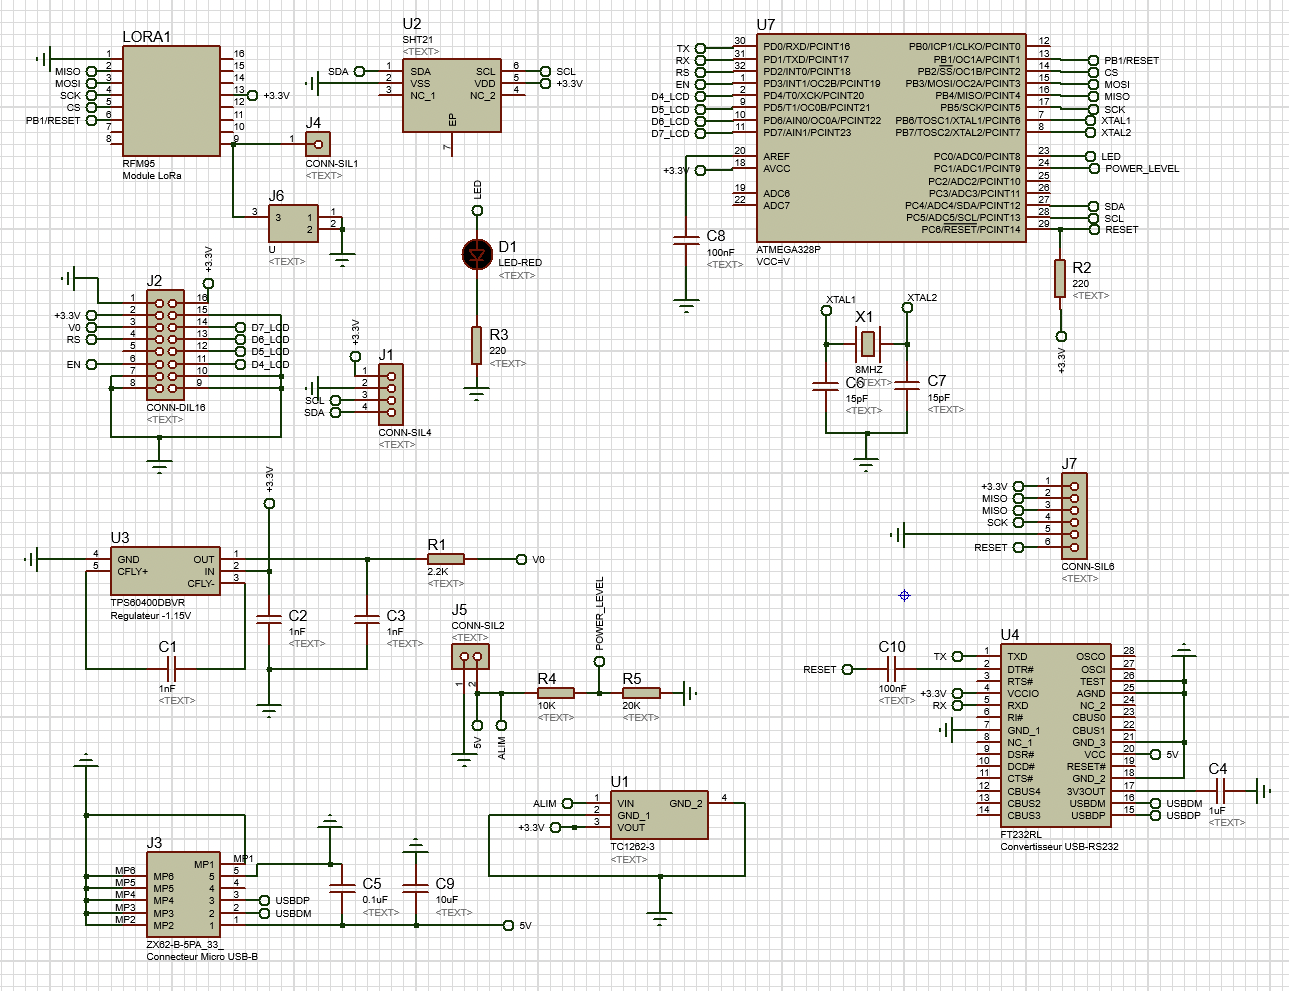
\includegraphics[width=1\textwidth]{img/proteus/schema.png}
                \caption{\label{fig:schema}Schéma de la carte capteur}  
            \end{center}  
        \end{figure}

        Pour la réalisation de la carte capteur, nous avons dans un premier temps récupéré l’ensemble des empreintes des composants. Pour certains, comme le module LORA, il a fallu réaliser son empreinte 
        (schématique et routage) à partir des données de la datasheet. \\
        Une fois les éléments rassemblés sur la feuille du schéma par groupe de fonction (Puissance, capteur, ATMEGA…), nous avons repris les datasheets des différents composants afin de définir les liaisons entre eux.

        

    \clearpage
    \section{Routage}

        \begin{figure}[!h]
            \centering
            \begin{minipage}{.48\linewidth}
                \begin{center}
                    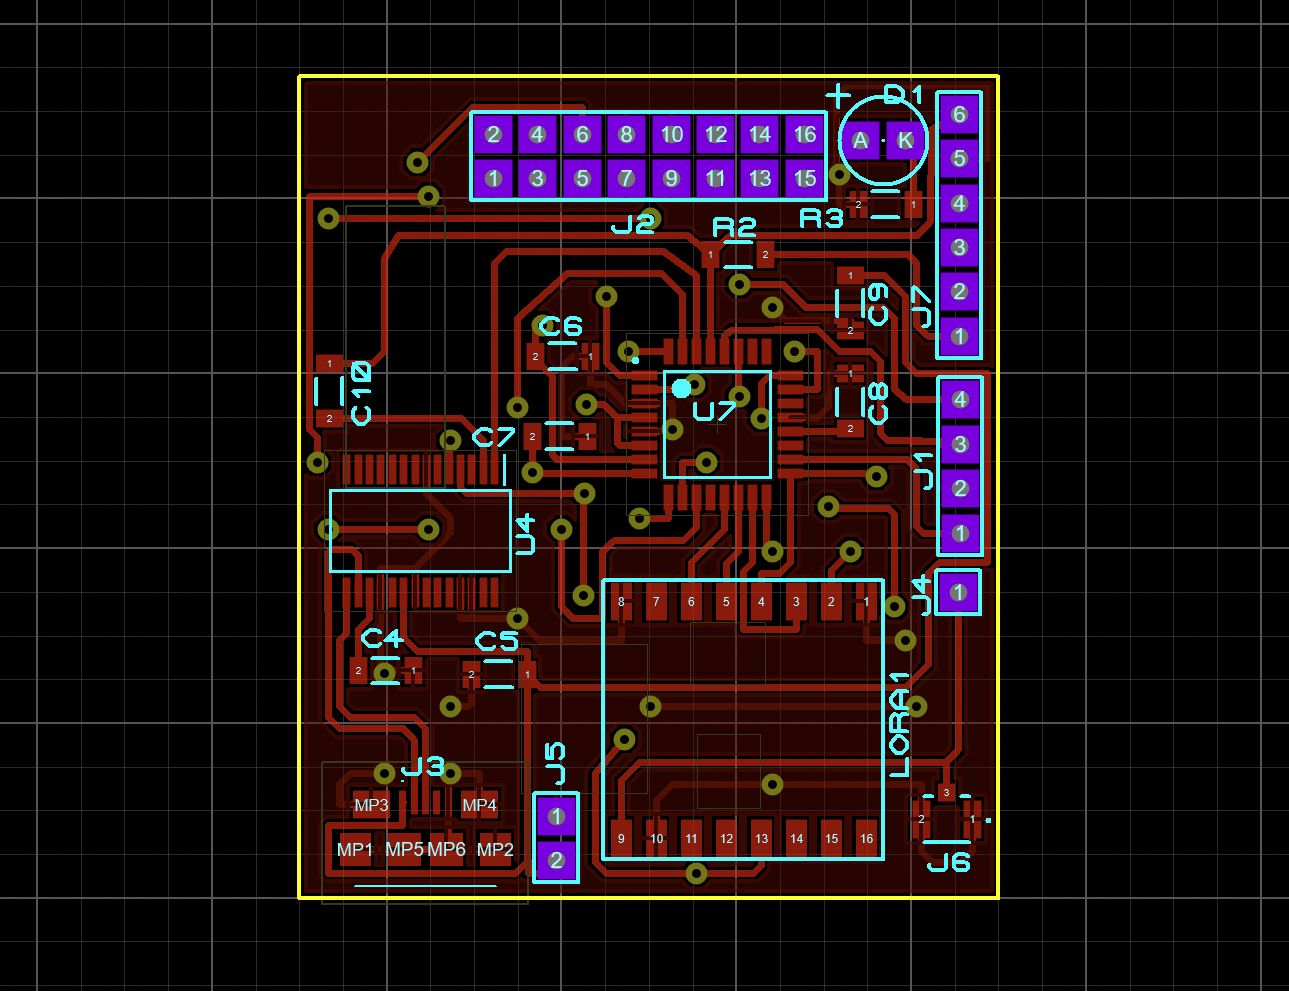
\includegraphics[width=1\textwidth]{img/proteus/routage_top.png}
                    \caption{\label{fig:routage_top}Routage de la carte capteur, couche supérieur}  
                \end{center}
            \end{minipage}\hfill
            \begin{minipage}{.48\linewidth}
                \begin{center}
                    \begin{center}
                        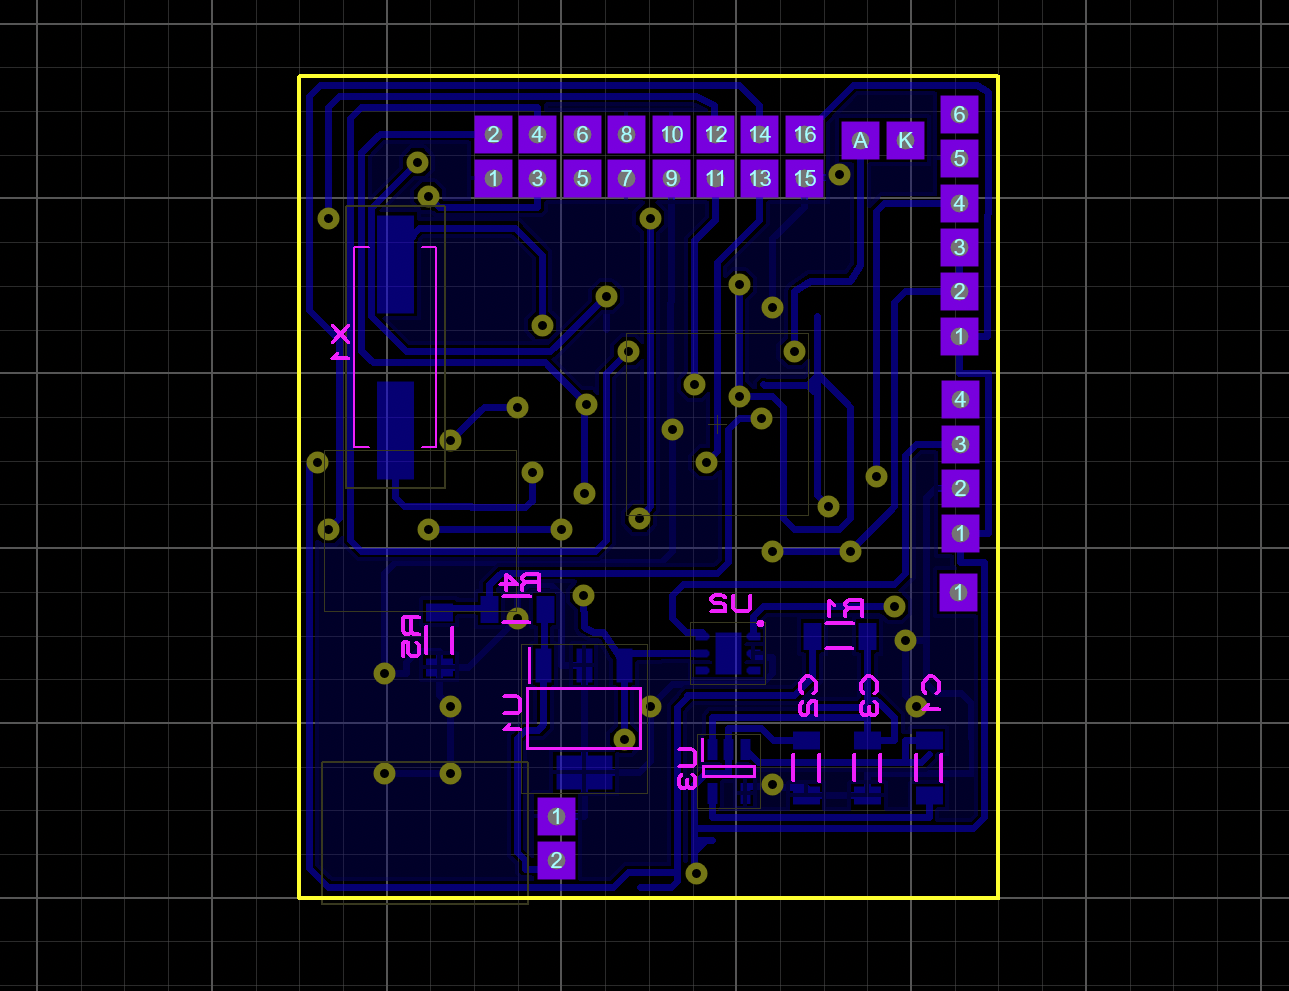
\includegraphics[width=1\textwidth]{img/proteus/routage_bottom.png}
                        \caption{\label{fig:routage_bottom}Routage de la carte capteur, couche inférieur}  
                    \end{center}
                \end{center}
            \end{minipage}
        \end{figure}

        Pour le routage, nous avons fais le choix de grouper nos composants de manière cohérente selon leur fonction. Cela nous a permis de réaliser un routage automatique sans avoir d’erreur. 
        Cependant le routage restait mal optimisé et nous avons donc repris un certain nombre de pistes afin de corriger les angles, limiter le nombre de via et vérifier leur placement sous les composants. \\
        Malheureusement, quelques détails nous ont échappé. L’empreinte du quartz n’était pas la bonne et le placement du LCD n’était pas optimal. Nous avons donc dû recommencer la démarche~: Routage auto/Modification/Vérification.  



    \section{Plan 3D}

        \begin{figure}[!h]
            \centering
            \begin{minipage}{.48\linewidth}
                \begin{center}
                    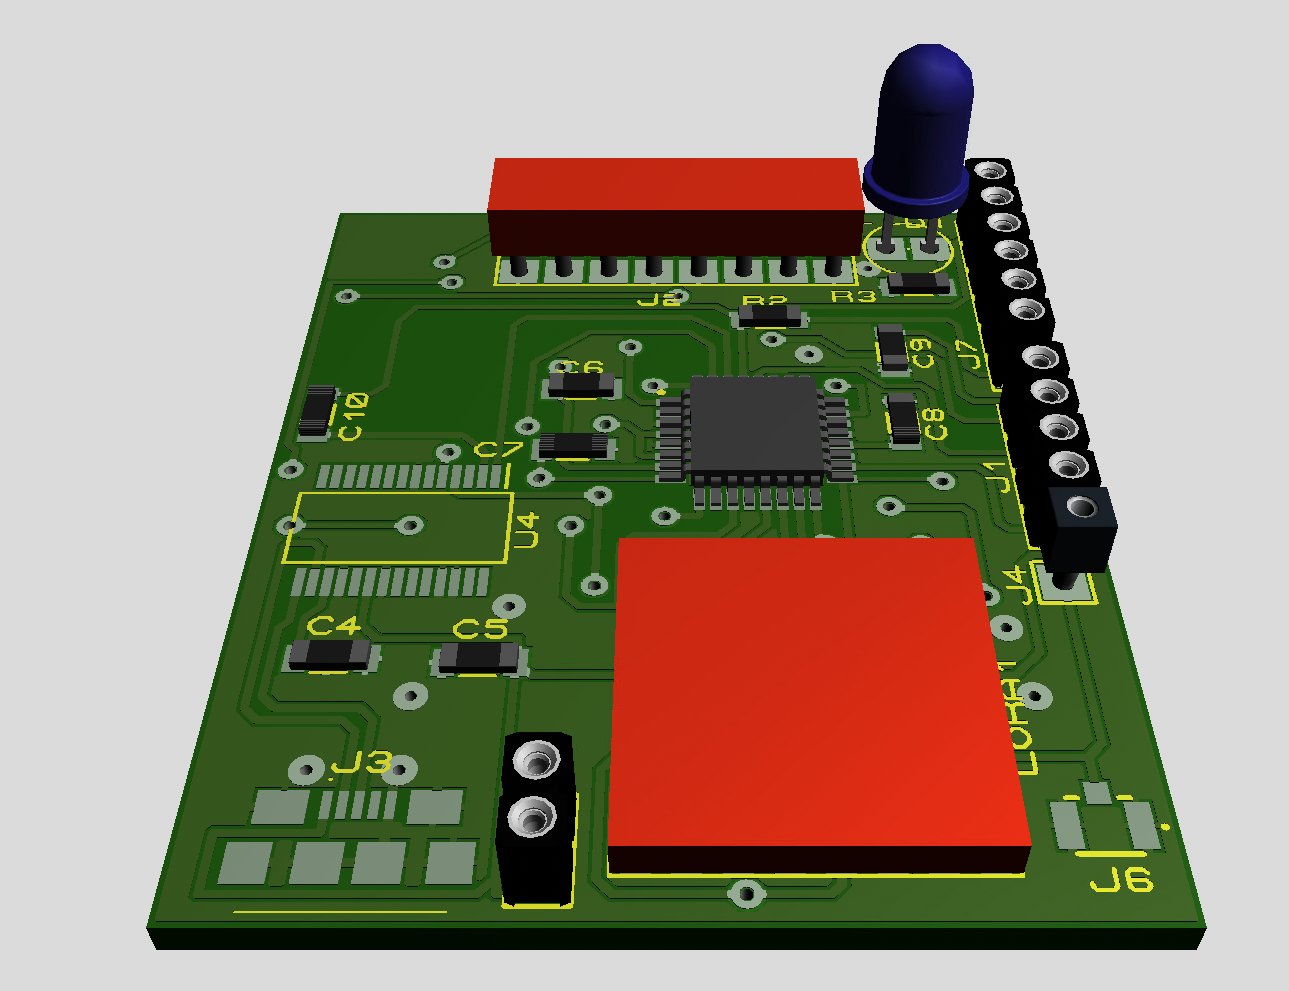
\includegraphics[width=1\textwidth]{img/proteus/3d_top.png}
                    \caption{\label{fig:3d_top}Vue 3D de la carte capteur, couche supérieur}  
                \end{center}
            \end{minipage}\hfill
            \begin{minipage}{.48\linewidth}
                \begin{center}
                    \begin{center}
                        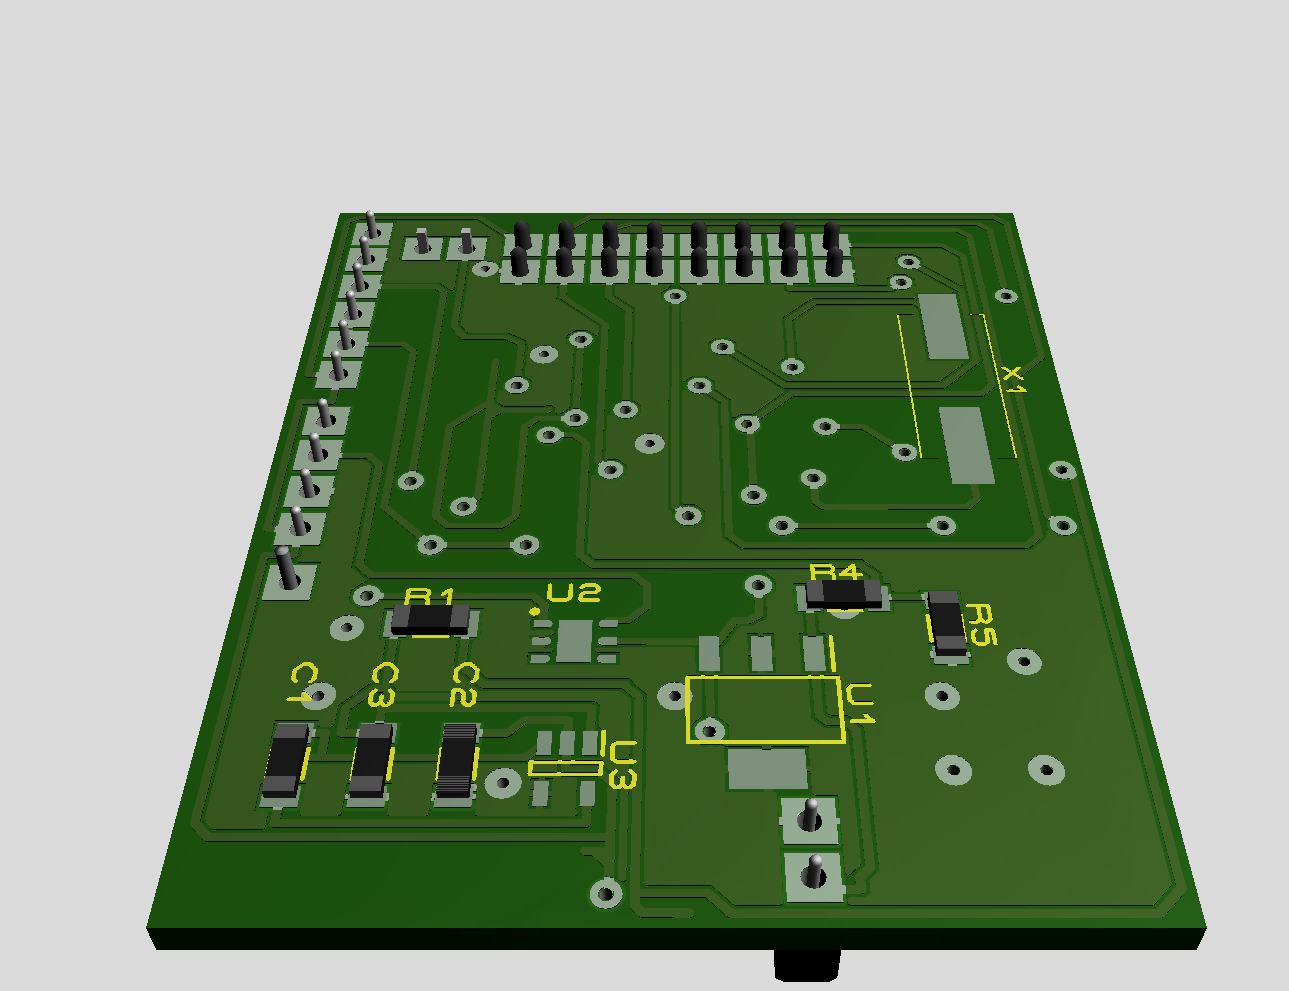
\includegraphics[width=1\textwidth]{img/proteus/3d_bottom.png}
                        \caption{\label{fig:3d_bottom}Vue 3D de la carte capteur, couche inférieur}  
                    \end{center}
                \end{center}
            \end{minipage}
        \end{figure}
